\documentclass{article}

\usepackage{amsmath}
\usepackage{amssymb}
\usepackage{enumerate}
\usepackage[spanish]{babel}
\usepackage{cancel}
\usepackage{caption}
\usepackage[margin=1.5in]{geometry}
\usepackage{graphicx}
\usepackage[utf8]{inputenc}
\usepackage{tcolorbox}
\usepackage{esint}
\usepackage{hyperref}
\hypersetup{
    colorlinks,
    citecolor=black,
    filecolor=black,
    linkcolor=black,
    urlcolor=black,
}

\renewcommand{\Bbb}{\mathbb}

\tcbuselibrary{theorems}

\title{Apuntes teórico-prácticos de Física I A (62.01) \\ Cátedra Menikheim \\ 1° C 2004}
\author{Darío Eduardo Ramos}

\definecolor{ududff}{rgb}{0.30196078431372547,0.30196078431372547,1}
\definecolor{cqcqcq}{rgb}{0.7529411764705882,0.7529411764705882,0.7529411764705882}

\begin{document}
\maketitle

\tableofcontents{}
\newpage

\section{Cinemática}

\subsection{Definiciones iniciales}

La \textbf{cinemática} es la rama de la física que describe el movimiento de los objetos sólidos sin considerar las causas que lo originan. 

El primer \textbf{modelo} que se adoptará para los cuerpos físicos a modelar será el de \textbf{punto material o partícula}: dichos cuerpos físicos serán considerados como sin volumen, pero sí con masa. Toda esa masa estará ``concentrada'' en el centro de masa del cuerpo, que será el punto que represente al objeto.

\textbf{Movimiento}: Un cuerpo será considerado en movimiento cuando cambie de posición a lo largo del tiempo respecto a un sistema de referencia considerado fijo o inercial. Más sobre esto último cuando se estudien los sistemas inerciales y no inerciales.

Cuando el cuerpo se desplaza desde una posición inicial dada por el vector $\overrightarrow{ r_i }$ a una posición final dada por el vector $\overrightarrow{ r_f }$, en un tiempo $\Delta t$, se definen las siguientes magnitudes vectoriales y escalares:

\begin{itemize}
\item \textbf{Vector desplazamiento:} $\overrightarrow{ \Delta r } = \overrightarrow{r_f} - \overrightarrow{r_i}$. Por como está definido, el vector $\overrightarrow{\Delta r}$ va de $\overrightarrow{r_i}$ hacia $\overrightarrow{r_f}$.
\item \textbf{Camino recorrido (escalar):}  $\Delta s$ = longitud del arco de trayectoria entre posición inicial y final.
\item \textbf{Vector velocidad media:} $\overrightarrow{v_m} = \frac{\overrightarrow{\Delta r}}{\Delta t}$
\item \textbf{Rapidez media (escalar):} $\overline{v} = \frac{\Delta s}{\Delta t}$
\item \textbf{Vector velocidad instantánea:}

\begin{equation}
\tcboxmath[colback=orange!25!white,colframe=orange]{
\overrightarrow{v} = \lim_{\Delta t \rightarrow 0} \frac{ \mathop{\overrightarrow{\Delta r}} }{\Delta t} = \frac{d\overrightarrow{r}}{\mathop{dt}}
}
\end{equation}

Nótese entonces que la velocidad instantánea es la derivada de la posición respecto al tiempo. Además, al ser $\overrightarrow{r}(t)$ una función vectorial del tiempo, $\overrightarrow{v}$ también lo es. Punto a punto, el vector $\overrightarrow{v}(t_0)$ es tangente a la curva de la trayectoria en el punto $\overrightarrow{r}(t_0)$ y su sentido es el del movimiento.
\item \textbf{Rapidez instantánea:}

\begin{equation}
v = \lim_{\Delta t \rightarrow 0} \frac{\Delta s}{\Delta t} = \frac{\mathop{ds}}{\mathop{dt}}
\end{equation}

\item \textbf{Vectores aceleración media e instantánea:}

\begin{equation}
\overrightarrow{a_m} = \frac{ \overrightarrow{ \Delta v } }{ \Delta t }
\end{equation}

\begin{equation}
\tcboxmath[colback=orange!25!white,colframe=orange]{
\overrightarrow{a} = \lim_{\Delta t \rightarrow 0} \frac{ \overrightarrow{ \Delta v } }{\Delta t} = \frac{ \mathop{d\overrightarrow{v}} }{ \mathop{dt} } = \frac{ \mathop{ d^2 \overrightarrow{r} } }{ \mathop{ dt^2 } }
}
\end{equation}

Cualquier cambio en el sentido, dirección o norma del vector velocidad indica que existe aceleración. Esto implica que en todo movimiento curvo hay aceleración no nula.

\end{itemize}

\subsection{Movimiento circular y movimiento curvo en general}

\subsubsection{Movimiento circular}

Algunas definiciones iniciales:

\begin{itemize}
\item \textbf{Velocidad angular (escalar):} $\omega = \frac{ \mathop{d\alpha} }{dt}$ = derivada del ángulo en función del tiempo.
\item \textbf{Ángulo en función del tiempo:} $\Delta \alpha = \omega \Delta t$
\item \textbf{Radianes:} $\alpha_{\mathop{rad}} = \frac{\text{longitud de arco}}{ \text{radio} }$
\item Relación entre $\omega$, el radio y la rapidez instantánea:

\begin{equation}
\alpha_{\mathop{rad}} = \frac{\text{longitud de arco}}{ \text{radio} } \Rightarrow \Delta \alpha = \frac{ \Delta s } {R} \Leftrightarrow \Delta s = \mathop{\Delta\alpha} \cdot R
\end{equation}

Reemplazando en la expresión general de la rapidez media:

\begin{equation}
\overline{v} = \frac{\Delta s}{\Delta t} \Rightarrow \overline{v} = \frac{\mathop{\Delta\alpha} \cdot R}{\Delta t} \Rightarrow v = \lim_{\Delta t \rightarrow 0} \underbrace{ \frac{\Delta \alpha}{\Delta t} }_{\omega} R \Rightarrow \tcboxmath[colback=orange!25!white,colframe=orange]
{ v = \omega R }
\end{equation}

De esta igualdad se puede concluir que si $\omega$ es constante, la rapidez instantánea también. Esto no aplica al vector velocidad, que tendrá norma constante, pero dirección variable.
\end{itemize}

\subsubsection{El vector velocidad}

Considerando $\overrightarrow{\omega}$ como un vector perpendicular, instante a instante, al plano del movimiento, se puede demostrar que para todo movimiento circular:

\begin{equation}
\tcboxmath[colback=orange!25!white,colframe=orange]{
\overrightarrow{v} = \overrightarrow{\omega} \times \overrightarrow{r}
}
\end{equation}

En esta igualdad, $\overrightarrow{r}$ es el vector posición. Dado que el sistema de referencia puede ser cartesiano o intrínseco, en ambos casos $\overrightarrow{r}$ se relaciona con el radio, aunque su expresión sea diferente.

Recuérdese que el vector resultado del producto vectorial es ortogonal a ambos vectores multiplicados a la vez. En este caso, $\overrightarrow{v}$ es ortogonal a $\overrightarrow{\omega}$ y también es ortogonal a $\overrightarrow{r}$. Además, el sentido de $\overrightarrow{v}$ está dado por la regla de la mano derecha.

\subsubsection{Coordenadas intrínsecas}

\begin{figure}[ht]
\centering
\caption{Coordenadas intrínsecas}
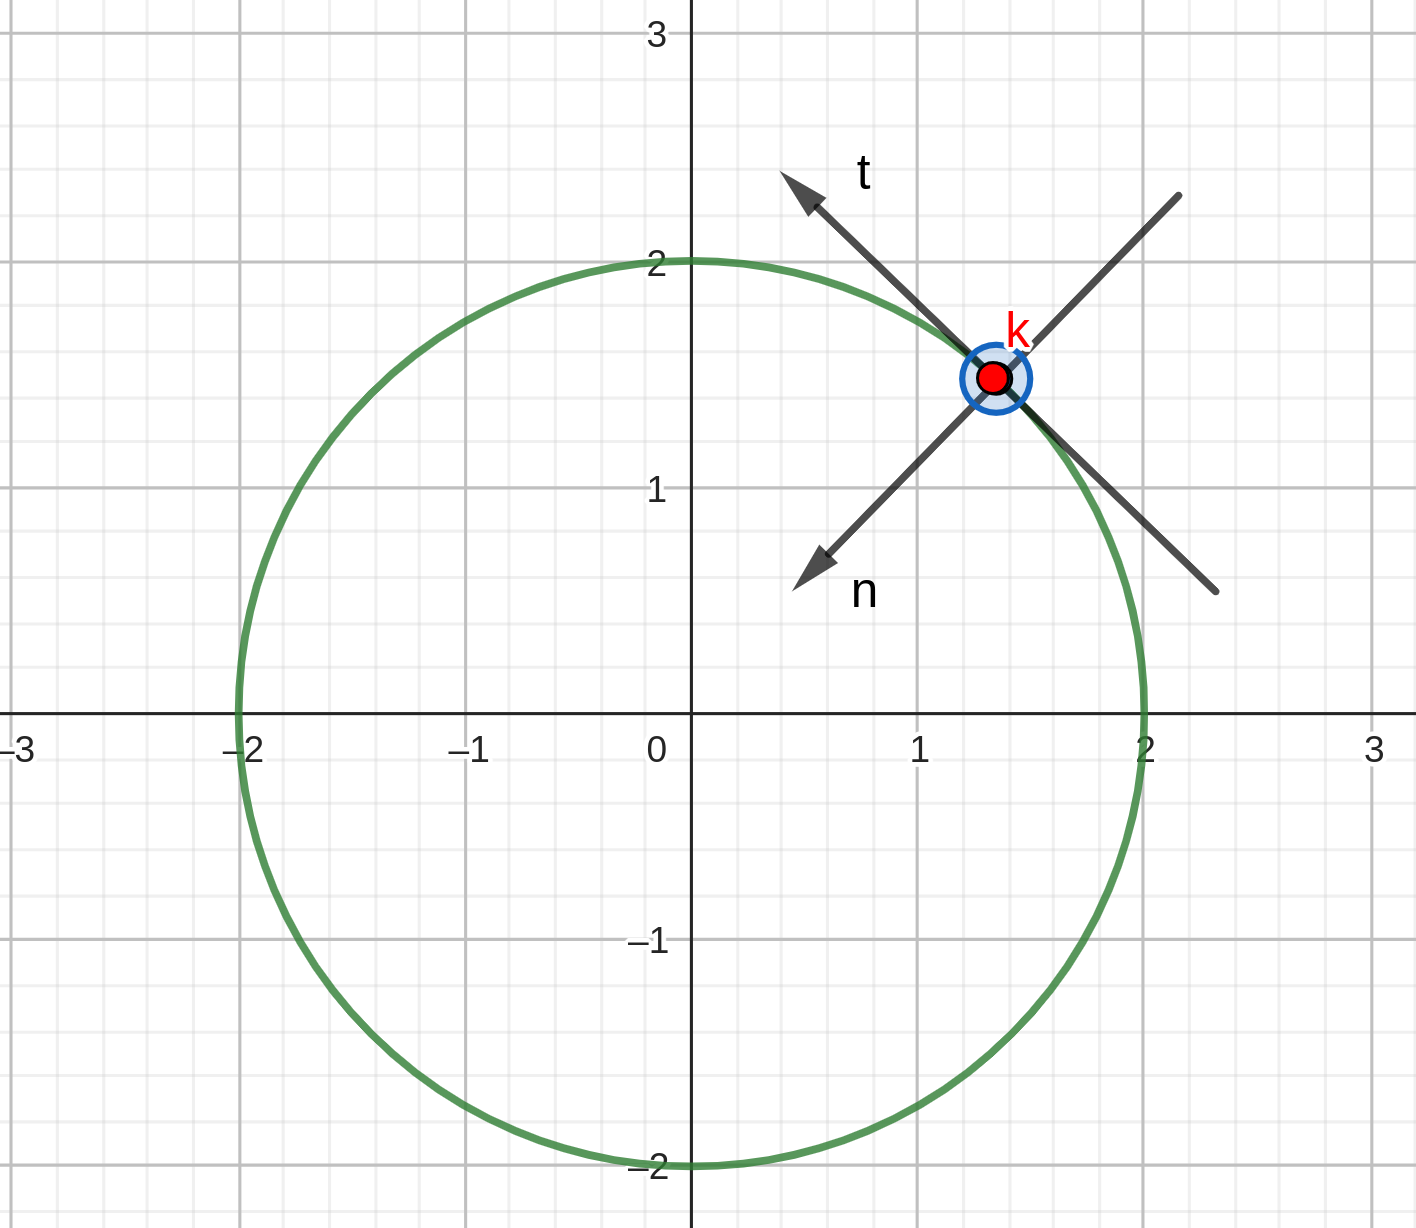
\includegraphics[scale=1]{../../common/img/62.01/theory/01-kinematics-intrinsic-coords.png}
\label{fig:intrinsicCoords}
\end{figure}

Obsérvese la figura \ref{fig:intrinsicCoords}. Para un instante determinado, el eje tangente $t$ se define positivo en el sentido de la velocidad. En cuanto al eje normal $n$, es positivo en el sentido de la concavidad, o sea hacia la parte interior del círculo. Finalmente, el eje binormal $k$, es positivo en el sentido de la aceleración angular $\gamma$. Es importante entender que este sistema de referencia es relativo a un instante específico de tiempo: para cada instante de tiempo, los ejes serán diferentes.

Con esta terna de ejes, resulta, si se denotan el radio del círculo con $R$, y los versores de los ejes con $\check{t}$, $\check{n}$ y $\check{k}$:

\begin{subequations}
\begin{align}
\overrightarrow{r} &= -R \check{n} \\
\overrightarrow{v} &= \omega R \check{t} \\
\overrightarrow{a_{\mathop{tg}}} &= \pm \gamma R \check{t} \\
\overrightarrow{a_{n}} &= \omega v \check{n}
\end{align}
\end{subequations}

Además, $R = ||\overrightarrow{r}||$ y $\gamma = ||\overrightarrow{\gamma}||$. Ahora bien, ¿de dónde salieron las expresiones de la aceleración tangencial y la aceleración normal? De derivar la velocidad. Ahora bien, al hacer eso, se utiliza el resultado de que la derivada de un producto vectorial sigue la misma regla que la derivada del producto de funciones. Verbigracia:

\begin{equation}
\overrightarrow{v} = \overrightarrow{\omega} \times \overrightarrow{r} \wedge \overrightarrow{a} = \frac{\mathop{d\overrightarrow{v}}}{\mathop{dt}} \Rightarrow \overrightarrow{a} = \underbrace{ \frac{\mathop{d\overrightarrow{\omega}}}{\mathop{dt}} }_{\overrightarrow{\gamma}} \times \overrightarrow{r} + \overrightarrow{\omega} \times \underbrace{ \frac{\mathop{d\overrightarrow{r}}}{\mathop{dt}} }_{\overrightarrow{v}}
\end{equation}

Resulta entonces:

\begin{equation}
\tcboxmath[colback=orange!25!white,colframe=orange, title=acelerac. en mov. circ.]{
\overrightarrow{a} = \underbrace{ \overrightarrow{\gamma} \times \overrightarrow{r} }_{\overrightarrow{a_{\mathop{tg}}}} + \underbrace{ \overrightarrow{\omega} \times \overrightarrow{v} }_{\overrightarrow{a_n}}
}
\end{equation}

En un movimiento circular, tanto $\overrightarrow{\omega}$ como $\overrightarrow{\gamma}$ jamás cambian su dirección, aunque sí puede cambiar su norma o su sentido.

Dado que $\overrightarrow{a_n}$ suele ser de especial interés por estar asociada a las fuerzas centrífugas, es de interés su norma:

\begin{equation}
a_n = ||\overrightarrow{a_n}|| = \omega v = \omega^2 R = \frac{v^2}{R}
\end{equation}

\subsubsection{Movimiento curvo generalizado}

Todo movimiento curvo puede ser analizado como la unión de movimiento circulares instantáneos, donde el radio es variable. Además, pasa a llamarse \textbf{radio de curvatura} y se denota con la letra $\rho$. Utilizando coordenadas intrínsecas, resulta:

\begin{equation}
\tcboxmath[colback=orange!25!white,colframe=orange]{
\overrightarrow{v} = \omega \rho \check{t}
}
\end{equation}

\begin{equation}
\tcboxmath[colback=orange!25!white,colframe=orange]{
\overrightarrow{a} = \underbrace{ \pm \gamma \rho \check{t} }_{\overrightarrow{a_{\mathop{tg}}}} + \underbrace{ \omega v \check{n} }_{\overrightarrow{a_n}}
}
\end{equation}

En este escenario generalizado, $\rho$ debe deducirse geométricamente, aunque esa no es la única forma de calcularlo. Por otro lado, puede decirse que $\overrightarrow{a_{\mathop{tg}}}$ está asociado a cambios en la norma de $\overrightarrow{v}$, en tanto $\overrightarrow{a_n}$ está asociado a cambios de dirección.

\subsection{Utilizando el cálculo integral}

Recordando que $\overrightarrow{v} = \frac{ \mathop{d \overrightarrow{r}} }{ \mathop{dt} }$ y $\overrightarrow{a} = \frac{ \mathop{d^2 \overrightarrow{r}} }{ \mathop{dt^2} }$, es posible utilizar el cálculo integral para hallar la magnitud original si se conoce su derivada. Esto ocurre siempre que dos magnitudes se relacionan a través de la derivada. Por ejemplo:

\begin{equation}
v_x = \frac{ \mathop{dx} }{ \mathop{dt} } \Rightarrow \mathop{ dx } = v_x \cdot \mathop{ dt } \Rightarrow \int_{x_0}^x \mathop{ dx } = \int_{t_0}^t v_x \cdot \mathop{ dt } \Rightarrow x - x_0 = \int_{t_0}^t v_x \cdot \mathop{ dt }
\end{equation}

Nótese que esto requiere conocer un punto de referencia $x_0 = r_x(t_0)$. Esta misma idea puede aplicarse para obtener la velocidad a partir de la aceleración.

\subsection{Calculando el radio de curvatura}

\begin{figure}[ht]
\centering
\caption{Radio de curvatura $\rho$}
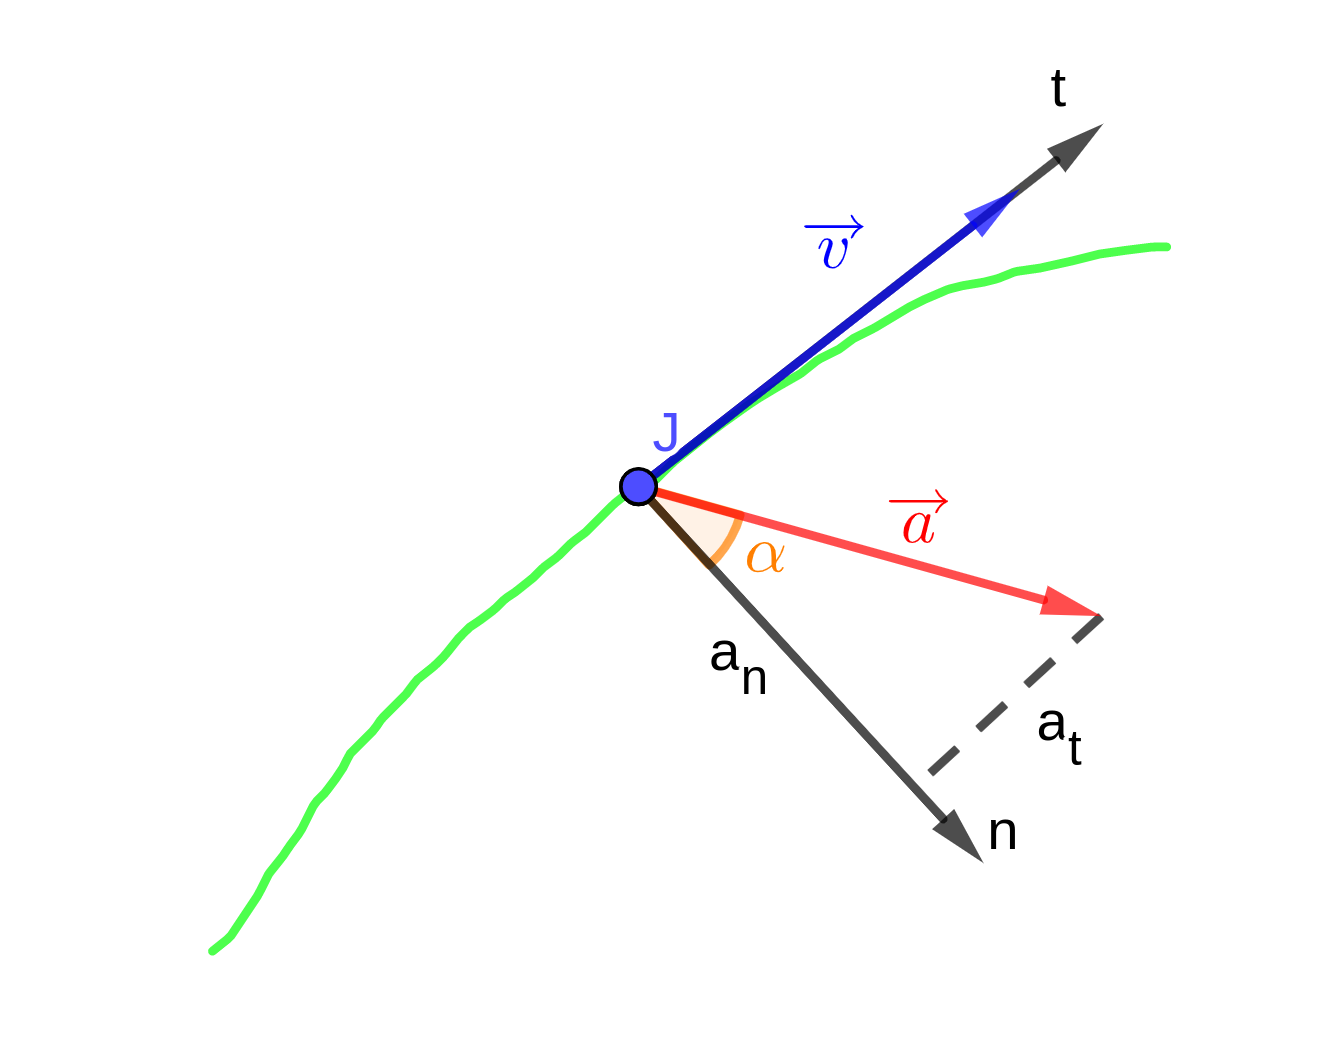
\includegraphics[scale=1.3]{../../common/img/62.01/theory/02-kinematics-rho.png}
\label{fig:rho}
\end{figure}

En base a la figura \ref{fig:rho}, dada la trayectoria, para calcular $\rho$ es necesario conocer la velocidad y la aceleración. Ello suele ser más directo utilizando un sistema de coordenadas intrínseco. En cuanto a $\alpha$, se deduce geométricamente. Con esos datos obtenidos, resulta:

\begin{subequations}
\begin{align}
a &= ||\overrightarrow{a}|| \\
a_n &= a \cos \alpha \wedge a_n = \frac{v^2}{\rho}
\end{align}
\end{subequations}

Finalmente:

\begin{equation}
\tcboxmath[colback=orange!25!white,colframe=orange]{
\rho = \frac{v^2}{a_n}
}
\end{equation}

\subsection{Movimiento relativo}

\subsubsection{Traslación}

\begin{figure}[ht]
\centering
\caption{Movimiento relativo - traslación}
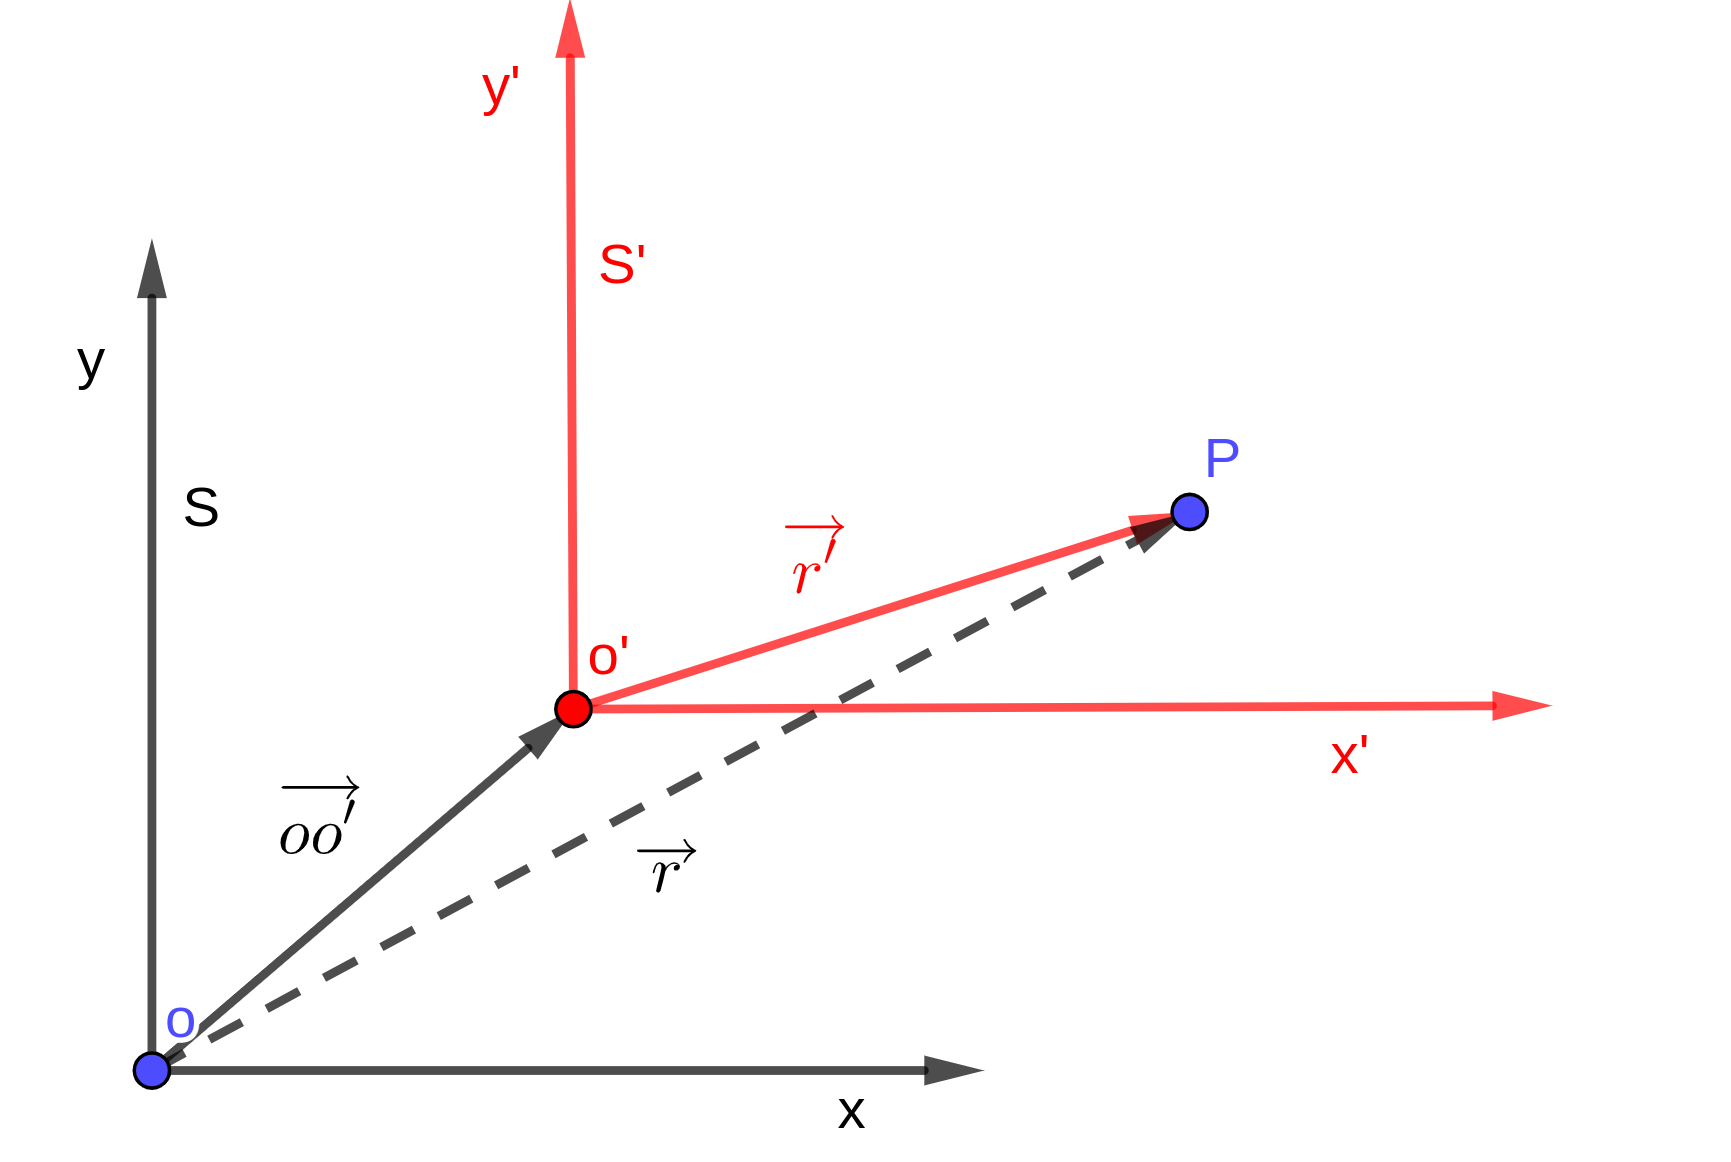
\includegraphics[scale=1.3]{../../common/img/62.01/theory/03-kinematics-rel-mov-tra.png}
\label{fig:relMovTra}
\end{figure}

En la figura \ref{fig:relMovTra}, se tiene un sistema de coordenadas $S$ que se considera fijo, y otro sistema $S'$ que se mueve respecto a $S$, pero sólo con traslación. Instante a instante, al no haber rotación, los ejes $x$ y $x'$ son paralelos en todo instante, al igual que $y$ e $y'$. Ello garantiza la siguiente igualdad vectorial, para todo tiempo $t$:

\begin{equation}
\overrightarrow{r} = \overrightarrow{oo'} + \overrightarrow{r'}
\end{equation}

\begin{itemize}
\item $\overrightarrow{r}$: Posición respecto al sistema fijo (posición absoluta).
\item $\overrightarrow{oo'}$: Posición del sistema móvil respecto al fijo (posición de arrastre). No perder de vista que esta magnitud también varía a lo largo del tiempo.
\item $\overrightarrow{r'}$: Posición respecto al sistema móvil (posición relativa).
\end{itemize}

Derivando miembro a miembro, resulta:

\begin{equation}
\tcboxmath[colback=orange!25!white,colframe=orange]{
\overrightarrow{v_{abs}} = \overrightarrow{v_{arr}} + \overrightarrow{v_{rel}}
}
\end{equation}

Derivando por segunda vez:

\begin{equation}
\tcboxmath[colback=orange!25!white,colframe=orange]{
\overrightarrow{a_{abs}} = \overrightarrow{a_{arr}} + \overrightarrow{a_{rel}}
}
\end{equation}

\subsubsection{Rotación}

\begin{figure}[ht]
\centering
\caption{Movimiento relativo - rotación}
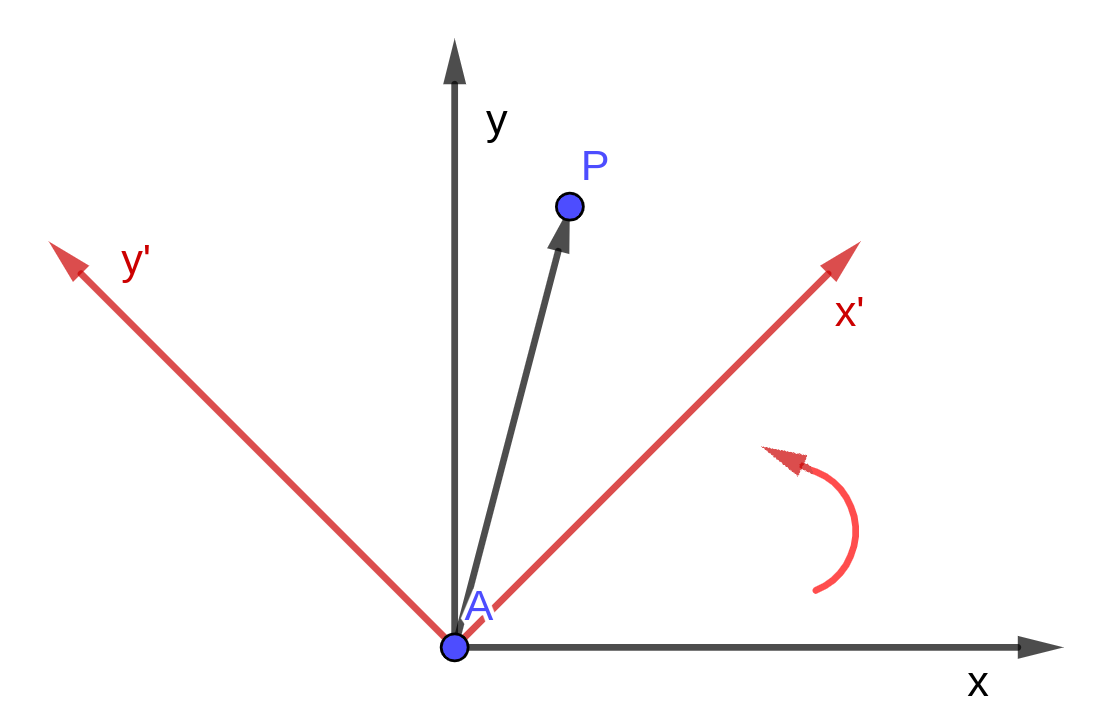
\includegraphics[scale=1.3]{../../common/img/62.01/theory/04-kinematics-rel-mov-rot.png}
\label{fig:relMovRot}
\end{figure}

En la figura \ref{fig:relMovRot}, el sistema $S'$ rota en sentido antihorario, sin transladarse, respecto al sistema $S$. Si se denota al versor $\check{i}$ como asociado al eje $x$, $\check{j}$ al eje $y$, y sus versiones primadas asociadas a los ejes de $S'$, es posible plantear:

\begin{subequations}
\begin{align}
\overrightarrow{r} &= x \check{i} + y \check{j} \\
\overrightarrow{r'} &= x' \check{i'} + y' \check{j'}
\end{align}
\end{subequations}

Derivando $\overrightarrow{r}$ respecto al tiempo, se obtiene $\overrightarrow{v_{abs}}$ de manera directa. Ahora bien, derivar $\overrightarrow{r'}$ no es tan directo, porque la posición de los versores primados varía a lo largo del tiempo. Aplicando la regla del producto, resulta:

\begin{equation}
\frac{ \mathop{ \overrightarrow{dr'} } }{ \mathop{dt} } = \frac{ \mathop{dx'} }{ \mathop{dt} } \check{i'} + x' \frac{ \mathop{d\check{i}'} }{ \mathop{dt} } + \frac{ \mathop{dy'} }{ \mathop{dt} } \check{j'} + y' \frac{ \mathop{d\check{j}'} }{ \mathop{dt} }
\end{equation}

Para analizar qué son las derivadas de los versores, considérese la variación de posición de uno de ellos a lo largo del tiempo, entre dos instantes.

\begin{figure}[ht]
\centering
\caption{Movimiento relativo - rotación - versores}
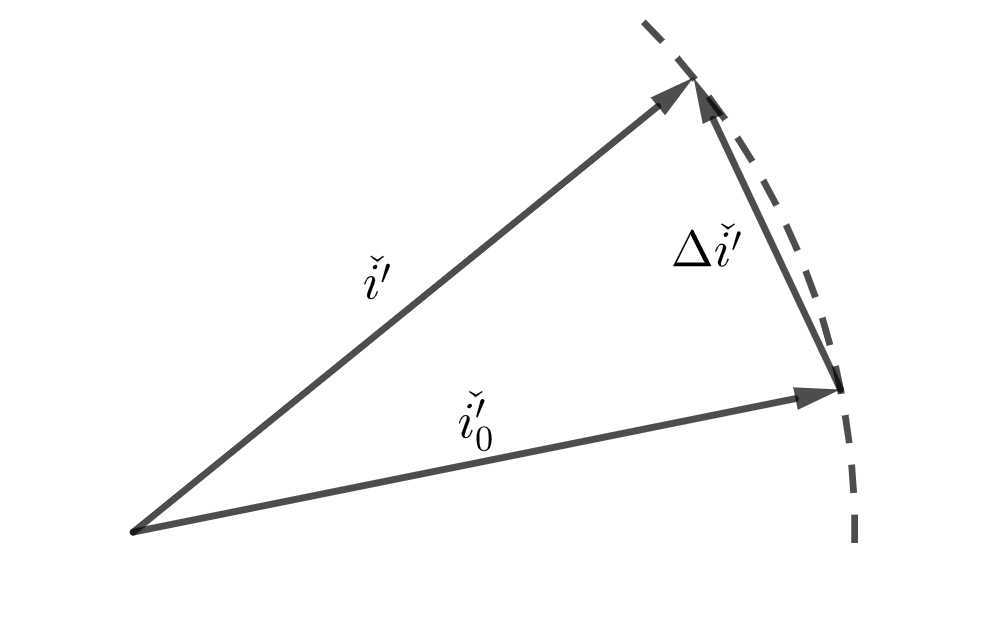
\includegraphics[scale=1.3]{../../common/img/62.01/theory/05-kinematics-rel-mov-rot-dv.png}
\label{fig:relMovRotDv}
\end{figure}

Observando la figura \ref{fig:relMovRotDv}, y considerando que la longitud de arco equivale al producto del ángulo por el radio, resulta, al tomar el límite:

\begin{equation}
\mathop{ d\check{i'} } = \mathop{ d\alpha } \underbrace{ ||\check{i'}|| }_{1} \check{j'}
\end{equation}

El hecho de que el diferencial de $\check{i'}$ tiene, como vector, la dirección $\check{j'}$ se observa geométricamente. Si se toma el límite, al acercarse $\check{i_0'}$ a $\check{i'}$, se observa que su dirección es ortogonal a la de $\check{i'}$. Como siguiente paso, en un abuso de notación, "dividiendo" miembro a miembro por $\mathop{dt}$, se tiene:

\begin{equation}
\frac{ \mathop{d \check{i'} } }{ \mathop{dt} } = \underbrace{ \frac{ \mathop{d\alpha} }{\mathop{dt}} }_{\omega} \check{j'}
\end{equation}

\begin{equation}
\tcboxmath[colback=orange!25!white,colframe=orange]{
\frac{ \mathop{d \check{i'} } }{ \mathop{dt} } = \omega \check{j'}
}
\end{equation}

Aplicando el mismo razonamiento para el versor $\check{j'}$, resulta entonces:

\begin{equation}
\tcboxmath[colback=orange!25!white,colframe=orange]{
\frac{ \mathop{d \check{j'} } }{ \mathop{dt} } = -\omega \check{i'}
}
\end{equation}

Es importante tener en cuenta que todo esto asume que el sentido de rotación de $S'$ es antihorario. Si el sentido fuera horario, las últimas dos igualdades tendrían el signo opuesto en $\omega$. Volviendo a la expresión de $\overrightarrow{r'}$:

\begin{subequations}
\begin{align}
\frac{ \mathop{ \overrightarrow{dr'} } }{ \mathop{dt} } &= \underbrace{ \frac{dx'}{dt} }_{v'_x} \check{i'} + x' \underbrace{ \frac{d\check{i'}}{dt} }_{\omega \check{j'}} + \underbrace{ \frac{dy'}{dt} }_{v'_y} \check{j'} + y' \underbrace{ \frac{d\check{j'}}{dt} }_{-\omega \check{i'}} \\
\frac{ \mathop{ \overrightarrow{dr'} } }{ \mathop{dt} } &= v'_x \check{i'} + x' \omega \check{j'} + v'_y \check{j'} + y' -\omega \check{i'}
\end{align}
\end{subequations}

Para el próximo paso, considérese el siguiente producto vectorial:

\begin{equation}
\overrightarrow{\omega} \times \overrightarrow{r'} = \det \begin{pmatrix}
\check{i'} & \check{j'} & \check{k'} \\
0 & 0 & \omega \\
x' & y' & 0
\end{pmatrix} = -y' \omega \check{i'} + x' \omega \check{j'}
\end{equation}

Reemplazando:

\begin{equation}
\frac{d\overrightarrow{r'}}{dt} = \underbrace{ v'_x \check{i'} + v'_y \check{j'} }_{\overrightarrow{v_{rel}}} + \underbrace{ \overrightarrow{\omega} \times \overrightarrow{r'} }_{?}
\end{equation}

¿Qué representa el segundo término? Puede pensarse como la velocidad de rotación del sistema móvil $S'$ respecto al sistema fijo $S$. Por ende, es la velocidad de arrastre.

Dado que $S'$ tiene siempre el mismo origen que $S$, en lo que concierne a $S$, $\overrightarrow{r} = \overrightarrow{r'}$ en todo instante. Por lo tanto, $\frac{d\overrightarrow{r}}{dt} = \frac{d\overrightarrow{r'}}{dt} = \overrightarrow{v_{abs}}$. Con lo que resulta finalmente:

\begin{equation}
\tcboxmath[colback=orange!25!white,colframe=orange]{
\vec{v}_{abs} = \underbrace{ v'_x \check{i'} + v'_y \check{j'} }_{\vec{v}_{rel}} + \underbrace{ \vec{\omega} \times \overrightarrow{r'} }_{\vec{v}_{arr}}
}
\end{equation}

Para obtener la aceleración, se deriva la velocidad. La derivada de $\vec{v}_{rel}$ es $\vec{a}_{rel}$, eso es trivial. Ahora bien, al derivar el producto vectorial del segundo término, se lo vuelve a expresar en términos de sus componentes, y se aplica la regla del producto:

\begin{equation}
\vec{a}_{abs} = \underbrace{ a'_x \check{i'} + a'_y \check{j'} }_{\vec{a}_{rel}} + \underbrace{ v'_x \omega \check{j'} - \omega v'_y \check{i'} }_{\vec{\omega} \times \vec{v'}} + \vec{\gamma} \times \vec{r} + \vec{\omega} \times \vec{v'}
\end{equation}

Finalmente, y sin perder de vista que este es el caso de sólo rotación:

\begin{equation}
\tcboxmath[colback=orange!25!white,colframe=orange]{
\vec{a}_{abs} = \vec{a}_{rel} + \underbrace{2 \vec{\omega} \times \vec{v'} }_{\text{ac. de Coriolis}} + \underbrace{ \vec{\gamma} \times \vec{r} }_{\vec{a}_{arr}}
}
\end{equation}

\section{Dinámica}

\subsection{Generalidades; 2da y 3ra leyes de Newton}

La dinámica es la rama de la física que estudia las causas del movimiento. Inicialmente, el modelo a seguir seguirá siendo el de partícula. Las causas serán interacciones (acciones mutuas) entre cuerpos, que pueden clasificarse de la siguiente manera:

\begin{itemize}
\item Fuertes: a nivel molecular. Pueden ser dentro del núcleo, o fuera del núcleo.
\item Débiles: producidas por campos. Esto incluye gravedad y electromagnetismo (por contacto o vínculo).
\end{itemize}

Nuestro estudio de la dinámica se centrará en las interacciones o fuerzas débiles.

\begin{itemize}
\item \textbf{Ley de las interacciones (3ra ley de Newton):} La característica principal de una interacción es la aparición de un par de fuerzas que actúan siempre en cuerpos distintos. Dichas fuerzas tienen igual dirección e intensidad, pero sentido opuesto.
\item \textbf{Vínculo}: Todo aquello que le quita libertad de movimiento a los cuerpos. Por ejemplo: mesa, piso, techo, soga, cadena, otro cuerpo.
\item \textbf{2da ley de Newton:} Para cada cuerpo, la suma vectorial de las fuerzas aplicadas sobre el mismo, o sea el vector fuerza resultante, equivale a la masa del cuerpo multiplicada por su vector aceleración. Matemáticamente:

\begin{equation}
\sum \vec{F} = \vec{F}_R = m \vec{a}
\end{equation}

En el contexto de la mecánica clásica, también llamada usualmente mecánica newtoniana, la masa se entiende como la cantidad de materia de un cuerpo, y es una magnitud escalar. En otros contexto como la mecánica cuántica, esa definición puede ser diferente. En esta materia, nos limitaremos a la definición newtoniana.

\item Pasos generales para resolver un problema de dinámica:

\begin{enumerate}
\item DCL: Diagrama de cuerpo libre. Indicar para cada cuerpo, las fuerzas que actúan como vectores.
\item Definir sistema de referencia, y sistema de coordenadas.
\item Para cada cuerpo, plantear la 2da ley de Newton, y resolver el sistema de ecuaciones resultante.
\end{enumerate}

\end{itemize}

\subsection{Rozamiento}

La fuerza de rozamiento aparece cuando una fuerza intenta cambiar el estado de movimiento de un cuerpo. Es una interacción: siempre habrá dos fuerzas iguales y opuestas en sentido. El vector $\vec{f}_r$ tiene, por convención, sentido opuesto al deslizamiento relativo entre las dos superficies.

El rozamiento puede ser \textbf{estático} o \textbf{dinámico}. El estático aplica cuando los cuerpos en contacto están sometidos a fuerzas no nulas, pero aún no hay movimiento relativo entre ambos. Para que empiece a haber movimiento, hay que vencer la fuerza de rozamiento estática. Por oposición, el rozamiento dinámico aparece cuando ya hay movimiento relativo entre los cuerpos. Como cabe esperar, los coeficientes de rozamiento son diferentes en ambos casos. Además, dependerán de los materiales de los cuerpos en contacto. Por ejemplo, hay coeficiente estático madera-madera, coeficiente estático madera-hierro, coeficiente dinámico madera-acero, etc.

\begin{figure}[ht]
\centering
\caption{Rozamiento}
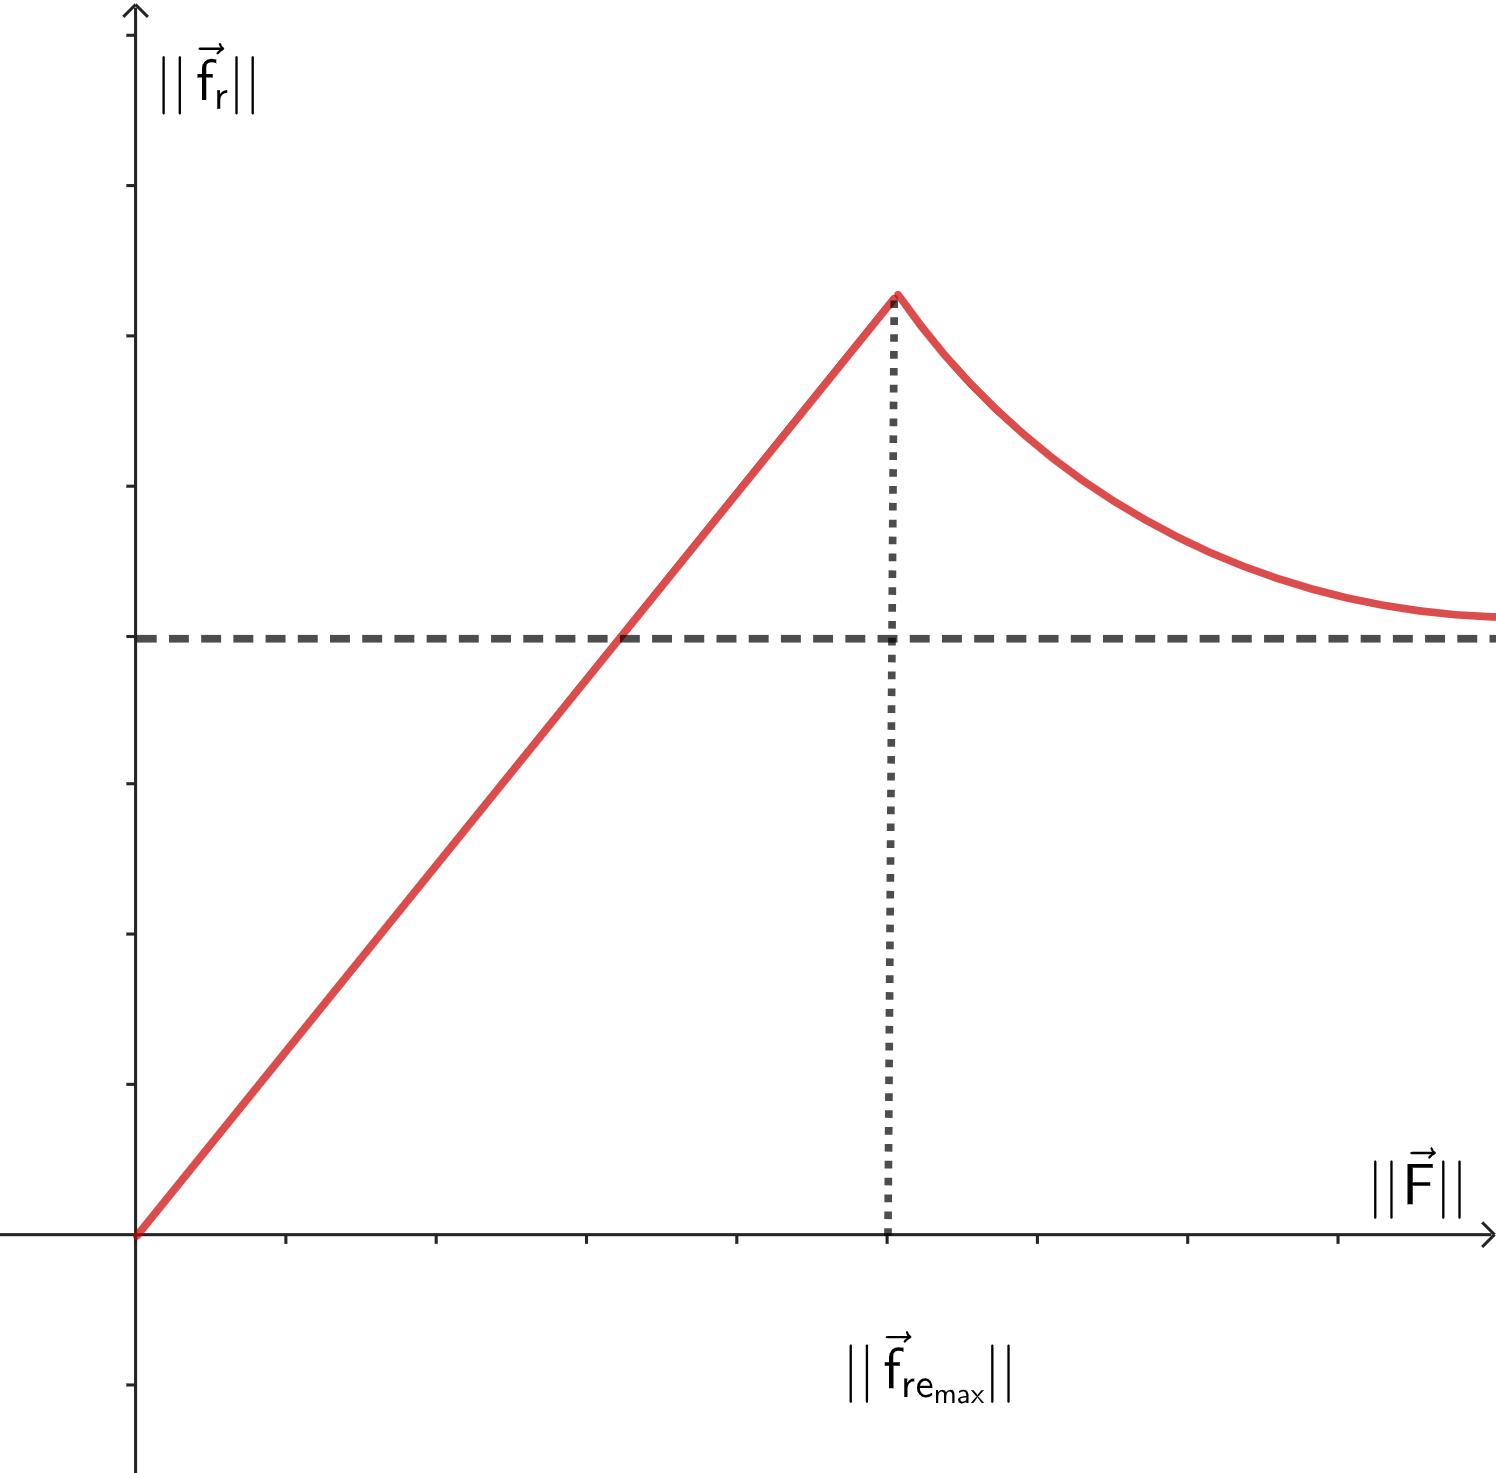
\includegraphics[scale=3.0]{../../common/img/62.01/theory/06-dynamics-friction.png}
\label{fig:friction}
\end{figure}

Si se grafica la intensidad de la fuerza aplicada al cuerpo contra la intensidad de la fuerza de rozamiento, suele seguir una curva como la de la figura \ref{fig:friction}. La intensidad de las fuerzas es lineal hasta que se llega a la intensidad máxima de rozamiento estático. Ese es el punto en que se pasa de rozamiento estático a dinámico. De ahí en adelante, la fuerza de rozamiento decae, pero tiende asintóticamente hacia una intensidad mínima. Vale decir, siempre habrá rozamiento.

De manera general, la intensidad de la fuerza de rozamiento está asociada a la intensidad de la normal y al coeficiente de rozamiento, según:

\begin{equation}
\tcboxmath[colback=orange!25!white,colframe=orange,title=Roz. estático]{
||\vec{f}_{re_{max}}|| = \mu_e ||\vec{N}||
}
\end{equation}

\begin{equation}
\tcboxmath[colback=orange!25!white,colframe=orange,title=Roz. dinámico]{
||\vec{f}_{rd}|| \approx \mu_d ||\vec{N}||
}
\end{equation}

En tanto se esté en rozamiento estático, $||\vec{f}_{re}|| \leq ||\vec{f}_{re_{max}}||$. El hecho de que una normal más intensa implica mayor fuerza de rozamiento estática máxima se condice con el hecho de que es más difícil poner en movimiento cuerpos de mayor masa. 

Si $||\vec{F}|| = ||\vec{f}_{re_{max}}||$, el cuerpo se mueve a velocidad constante. 

Por último, una forma intuitiva de calcular los coeficientes de rozamiento es pensar que $\mu \propto \frac{\text{ptos de contacto}}{\text{superficie}}$. Un par de superficies lisas tendrán un área de contacto casi igual a su superficie de contacto, y por ende tenderán a un coeficiente cercano a 1, que representa la ausencia de rozamiento. Por otro lado, un par de superficies más rugosas o disímiles entre sí tendrán menos puntos de contacto y por ende más fricción.

\subsection{Viscosidad}

Dado un cuerpo en movimiento dentro de un fluido, la viscosidad es una fuerza que se opone al movimiento del cuerpo. En particular, y en casos donde sea relevante, el aire puede ser considerado un fluido. Una forma básica de modelar la viscosidad es la siguiente:

\begin{equation}
\tcboxmath[colback=orange!25!white,colframe=orange,title=Viscosidad]{
\vec{F}_{rv} = -k \vec{v}
}
\end{equation}

El sufijo rv corresponde a un nombre alternativo de la fuerza viscosidad: resistencia viscosa. La constante $k$ depende del fluido, y $\vec{v}$ es, como cabe esperar, la velocidad del cuerpo. A continuación, se verá un ejemplo que combina rozamiento y viscosidad, y analiza el concepto de \textbf{velocidad crítica}.

Sea un cuerpo rectangular de masa $m$, modelado como partícula, sujeto a una fuerza externa conocida $\vec{F}$. Dicho cuerpo se encuentra apoyado sobre una superficie con rozamiento dinámico $\mu_{d}$, y dentro de un fluido con viscosidad $k$. Esta situación se grafica en la figura \ref{fig:viscosity}.

\begin{figure}[ht]
\centering
\caption{Viscosidad}
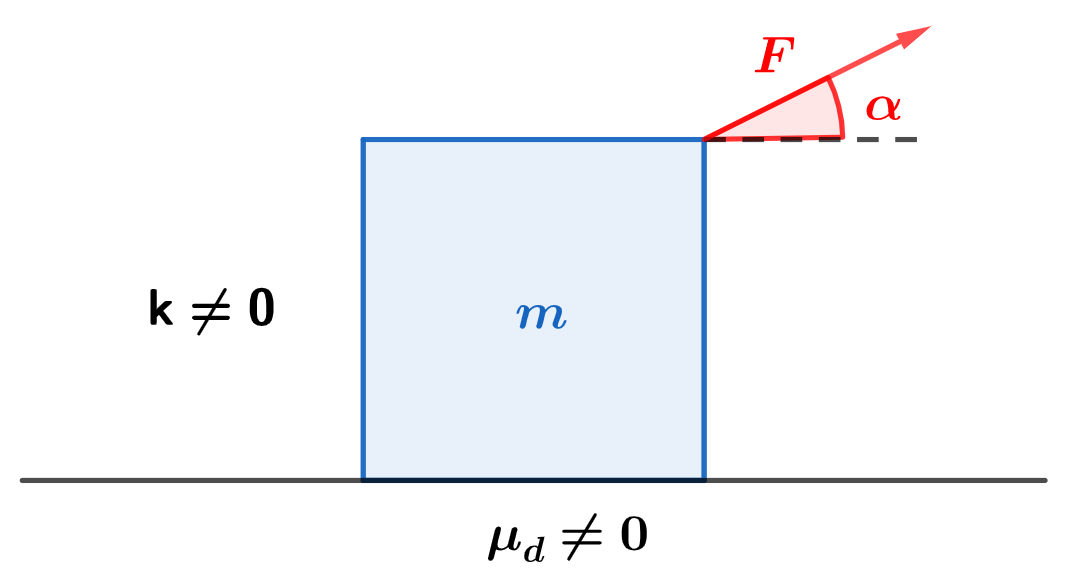
\includegraphics[scale=1.0]{../../common/img/62.01/theory/07-dynamics-viscosity-example.png}
\label{fig:viscosity}
\end{figure}

Modelando el cuerpo como partícula, se obtiene el diagrama de cuerpo libre de la figura \ref{fig:fbd}.

\begin{figure}[ht]
\centering
\caption{Viscosidad - DCL}
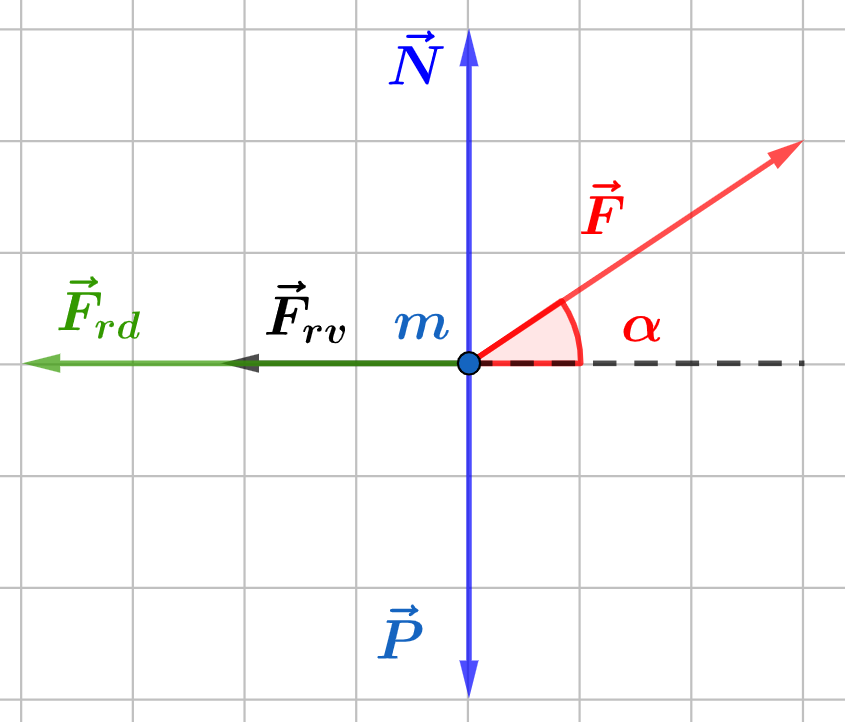
\includegraphics[scale=1.0]{../../common/img/62.01/theory/07-dynamics-viscosity-fbd.png}
\label{fig:fbd}
\end{figure}

Dado que el cuerpo está apoyado en un plano horizontal, y tiene una masa $m$, se plantean la fuerza peso $\vec{P}$, y la normal del plano horizontal $\vec{N}$. En color rojo se observa la fuerza externa $\vec{F}$. Dado que, para una partícula, dicha fuerza producirá un movimiento horizontal paralelo al plano, las fuerzas de rozamiento dinámico ($\vec{F}_{rd}$) y viscosidad ($\vec{F}_{rv}$) tienen vectores dirección opuestos a los del movimiento del objeto. Se dibujó $\vec{F}_{rd}$ como si tuviera mayor módulo que $\vec{F}_{rd}$ de manera arbitraria e ilustrativa; puede darse el caso opuesto, y ello se sabrá al resolver el sistema.

El segundo paso es definir un sistema de referencia. El mismo se define como un par de ejes cartesianos $x$ e $y$ con origen en la posición inicial del cuerpo.

El tercer y último paso es plantear la segunda ley de Newton para las dos dimensiones del problema. En este punto, se asume que la fuerza $F$ es tal que sólo produce movimiento horizontal en el cuerpo. Vale decir, la aceleración en la componente $y$ es nula. Teniendo esto en cuenta, resulta:

\begin{subequations}
\begin{align}
\textbf{x)} & \quad F \cos(\alpha) - k v - \mu_d N = m a \\
\textbf{y)} & \quad N - P + F \sin(\alpha) = 0
\end{align}
\end{subequations}

Despejando $N$ en la ecuación $\textbf{y)}$:

\begin{equation}
N = P - F \sin(\alpha)
\end{equation}

Reemplazando en la ecuación $\textbf{x)}$:

\begin{equation}
F \cos(\alpha) - k v - \mu_d (P - F \sin(\alpha)) = m a
\end{equation}

Si la fuerza $\vec{F}$ es constante en el tiempo, su módulo $F$ y el ángulo $\alpha$ también lo son. Restringiendo la solución a ese caso y recordando que $P$ es conocida por ser el producto de la masa $m$ por la constante $g$, la única incógnita que queda es la aceleración del cuerpo en función del tiempo, y su velocidad. Expresando la aceleración como la derivada de la velocidad respecto al tiempo, se obtiene la siguiente ecuación diferencial:

\begin{equation}
F [\cos(\alpha) + \mu_d \sin(\alpha)] - \mu_d P - k v = m \frac{\mathop{dv}}{\mathop{dt}}
\end{equation}

En esta ecuación, la incógnita es la función $v(t)$. Nótese que dicha ecuación es de variables separables, dado que es posible poner $t$ y $dt$ de un lado de la igualdad, y $v$ y $dv$ del otro.

\begin{equation}
\mathop{dt} = \frac{m}{-k v + F [\cos(\alpha) + \mu_d \sin(\alpha) - \mu_d P]}
\end{equation}

Integrando de ambos lados y haciendo el cambio de variable $u = $ todo el denominador, se llega a que:

\begin{equation}
v = C e^{-\frac{k}{m} t} + F [\cos(\alpha) + \mu_d \sin(\alpha) - \mu_d P]
\end{equation}

En esta expresión final de la velocidad, la constante $C$ es de integración y se calcula usando las condiciones iniciales del problema. Nótese que la solución tiene un término transitorio exponencial que depende sólo de la viscosidad y de la masa, y un término permanente constante que depende de la fuerza aplicada, el rozamiento dinámico, la masa del objeto y la aceleración de la gravedad. Este término permanente es lo que se conoce como \textbf{velocidad crítica}: a partir de cierto instante de tiempo, el término exponencial pasa a ser despreciable, y a fines prácticos, la velocidad del cuerpo se mantiene constante. Este valor de tiempo se conoce como \textbf{tiempo crítico}, y suele tomarse como $\frac{5k}{m}$. Esto surge de la regla práctica de que dada la exponencial decreciente $e^{\tau t}$, pasadas $5 \tau$ unidades de tiempo, la exponencial es, a fines prácticos, cero. Por último, nótese que como cabe esperar, el tiempo crítico depende de la viscosidad y la masa del cuerpo.

\subsection{Vínculos}

En el contexto de la mecánica clásica o newtoniana, los \textbf{vínculos} o \textbf{restricciones} describen condiciones que limitan o determinan el movimiento de los objetos o sistemas en estudio. Pueden observarse varios ejemplos de vínculos en la figura \ref{fig:constraints}. En dicha figura, los vectores de color rojo representan posibles fuerzas externas, y las flechas curvadas verdes en el caso de la rótula indican las dos posibles direcciones de movimiento de la misma. Por otro lado, en el caso del empotramiento, el cuerpo empotrado está totalmente fijo. Naturalmente, esto no contempla casos donde la fuerza sobre el cuerpo sea tan grande que lo doble o quiebre; no se modelarán ese tipo de casos en esta materia, y se asumirá que el cuerpo empotrado soportará las fuerzas a las que sea sometido.

\begin{figure}[ht]
\centering
\caption{Vínculos}
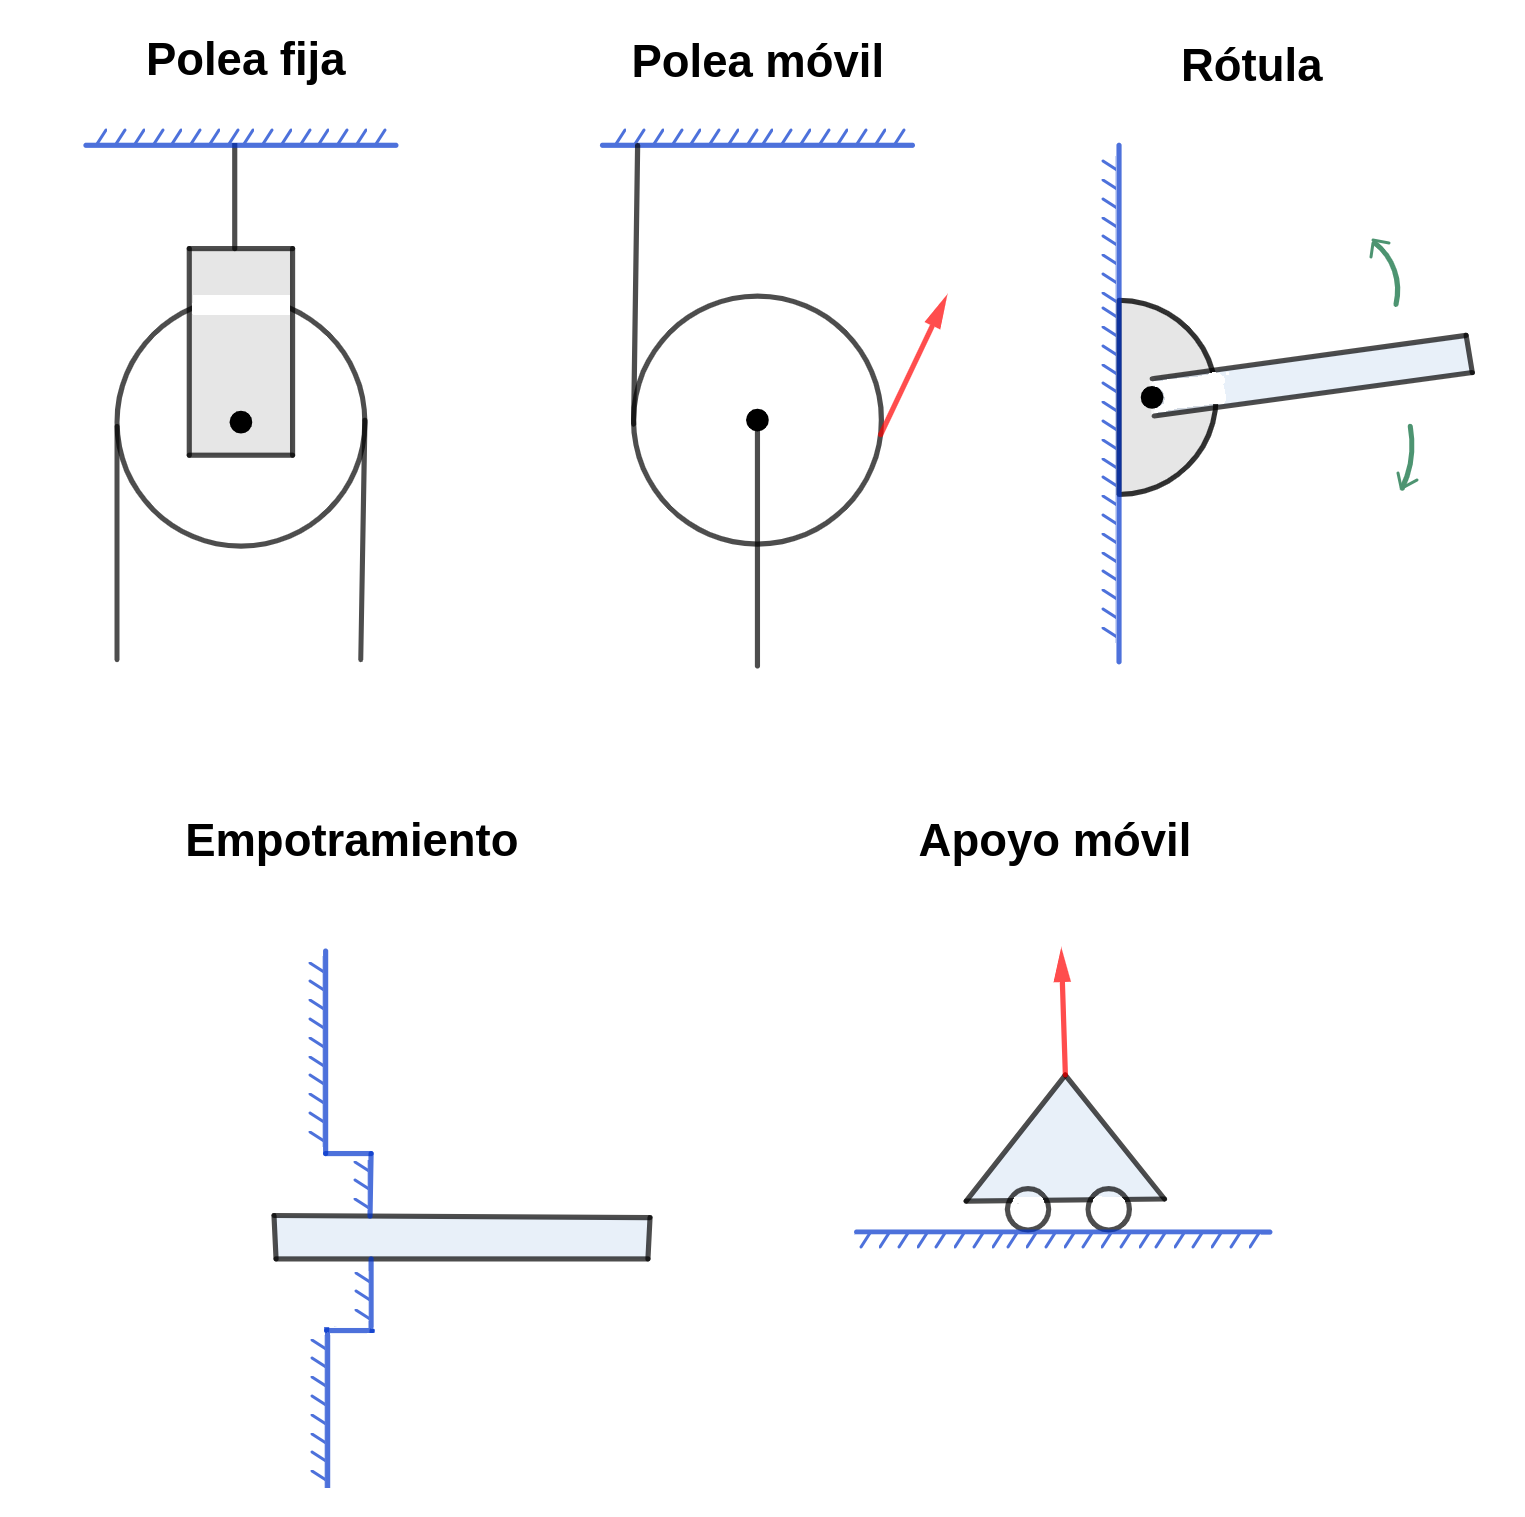
\includegraphics[scale=0.7]{../../common/img/62.01/theory/08-dynamics-constraints.png}
\label{fig:constraints}
\end{figure}

Otra consideración que se adoptará al lidiar con vínculos será la siguiente: las poleas, cadenas, cuerdas y demás cuerpos vinculados serán considerados inextensibles y de masa despreciable cuando su masa sea 10 veces menor que la de los demás cuerpos considerados. Este es un buen criterio general para sistemas mecánicos básicos.

\subsection{1ra ley de Newton: inercia}

Si la suma de fuerzas sobre un cuerpo es cero al menos en una dirección, en dicha dirección, si el cuerpo estaba en reposo permanecerá en reposo, y si se estaba moviendo continuará haciéndolo a velocidad constante. Recuérdese que para la suma de fuerzas también se utiliza el término \textbf{resultante}.

Si un sistema se mueve a velocidad constante, es equivalente a un \textbf{sistema inercial (SI)}. En cambio, si el sistema tiene una aceleración no nula, pasa a ser un \textbf{sistema no inercial (SNI)}.

Considérese el sistema de la figura \ref{fig:inertia}. Hay una barra de hielo apoyada sobre un camión. El camión tiene una aceleración no nula, y el rozamiento entre el hielo y el piso de la caja del camión es nulo.

\begin{figure}[ht]
\centering
\caption{Inercia - ejemplo}
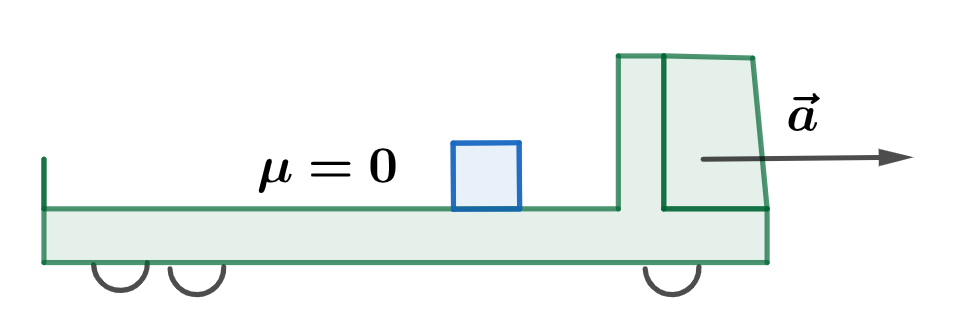
\includegraphics[scale=1.0]{../../common/img/62.01/theory/09-dynamics-inertia.png}
\label{fig:inertia}
\end{figure}

Si se observa sólo la barra de hielo tomando como referencia la tierra, la misma no se mueve: el camión avanzará y la barra resbalará hasta vincularse con el tope trasero de la caja del camión. Esto ocurre porque la tierra es un sistema inercial: para los fines de este problema, la tierra está en reposo y se cumple la 1ra ley, al menos hasta que la barra hace tope. Si se hiciera un diagrama de cuerpo libre de la barra de hielo en este caso, las únicas fuerzas serían el peso y la normal en la dirección y, y sumarían cero. En la dirección x no hay movimiento, al menos en el intervalo de interés (pre vínculo con tope trasero del camión).

Ahora bien, si se toma como sistema de referencia el camión, las fuerzas son las mismas, pero se observa un movimiento en la barra. Esto ocurre porque el sistema de referencia mismo está acelerado: es un \textbf{sistema de referencia no inercial (SRNI)}. Para que sigan valiendo las leyes de Newton, es preciso aplicar una fuerza ficticia a todo cuerpo del sistema. Dicha fuerza tendrá dirección opuesta a la aceleración del sistema, y su módulo será el producto de la masa del cuerpo en cuestión por el módulo de la aceleración del sistema. Para el caso de la barra, tomando como sistema de referencia el camión, el diagrama de cuerpo libre sería ahora el de la figura \ref{fig:inertia-example}.

\begin{figure}[ht]
\centering
\caption{Inercia - ejemplo - DCL}
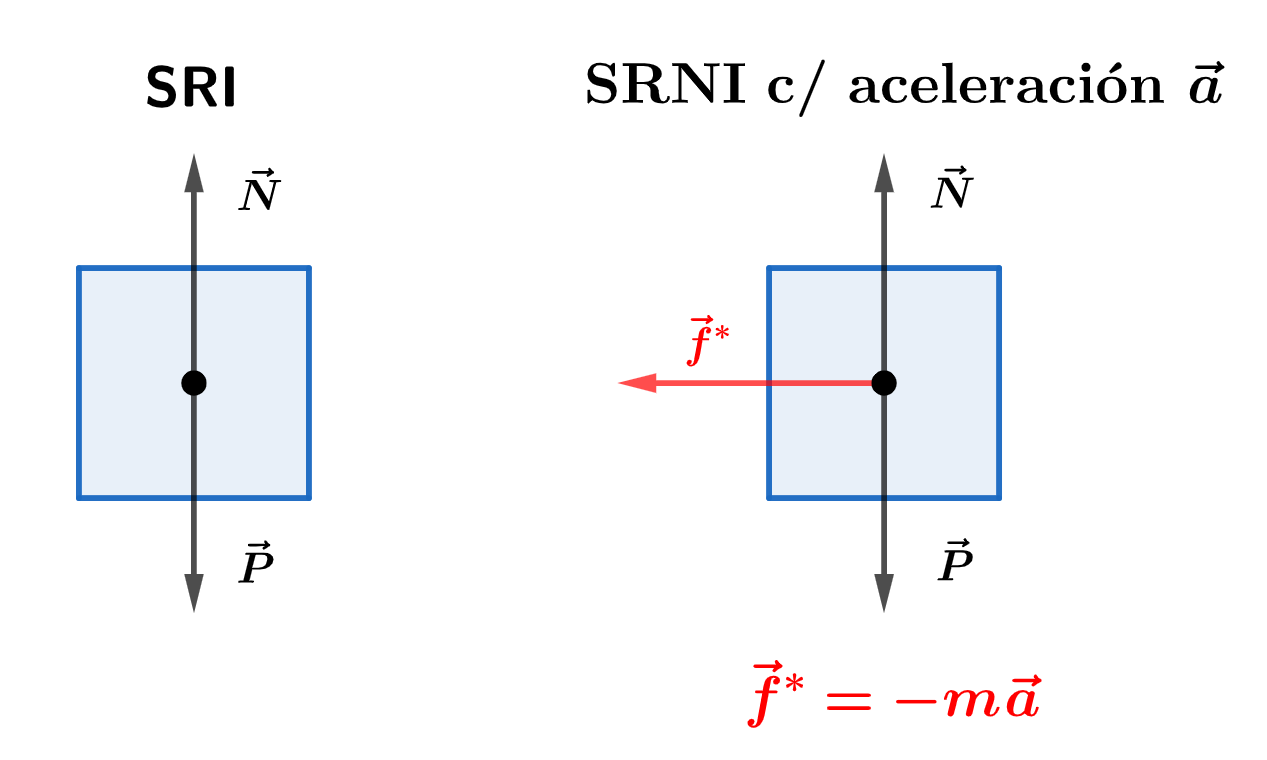
\includegraphics[scale=0.8]{../../common/img/62.01/theory/10-dynamics-inertia-example.png}
\label{fig:inertia-example}
\end{figure}

La fuerza ficticia $\vec{f}^{*}$ es la que justifica el movimiento observado en la barra de hielo cuando el sistema de referencia es el camión. Recuérdese que si hubiera más cuerpos, todos tendrían aplicada una fuerza ficticia proporcional a su masa.

\subsubsection{Péndulo cónico}

Éste es otro ejemplo de cómo un sistema puede verse como inercial o no inercial según el sistema de referencia adoptado. Observando el diagrama de la figura \ref{fig:conic-pendulum}, y asumiendo que no hay rozamiento u otros efectos que detengan el movimiento del péndulo, el cuerpo colgado de la cuerda realizará un movimiento circular en un plano horizontal. Esto requiere que la cuerda sea larga, flexible, sin masa e inextensible (que no se estire).

Si en primer lugar se toma como referencia la tierra, se tiene un sistema inercial. Concretamente, se define el eje x dentro del plano de movimiento y el eje y, perpendicular. Nótese que con este esquema, sólo se observa la posición del cuerpo en la proyección lateral del plano, no en las dos coordenadas que tendría si se observara el movimiento que realiza desde arriba. Con este sistema de referencia, fijo e inercial, y en las condiciones dadas, se observa movimiento y aceleración en la dirección x. En la dirección y, el peso del cuerpo es compensado por la componente y de la tensión en la cuerda.

\begin{figure}[ht]
\centering
\caption{Péndulo cónico - SI}
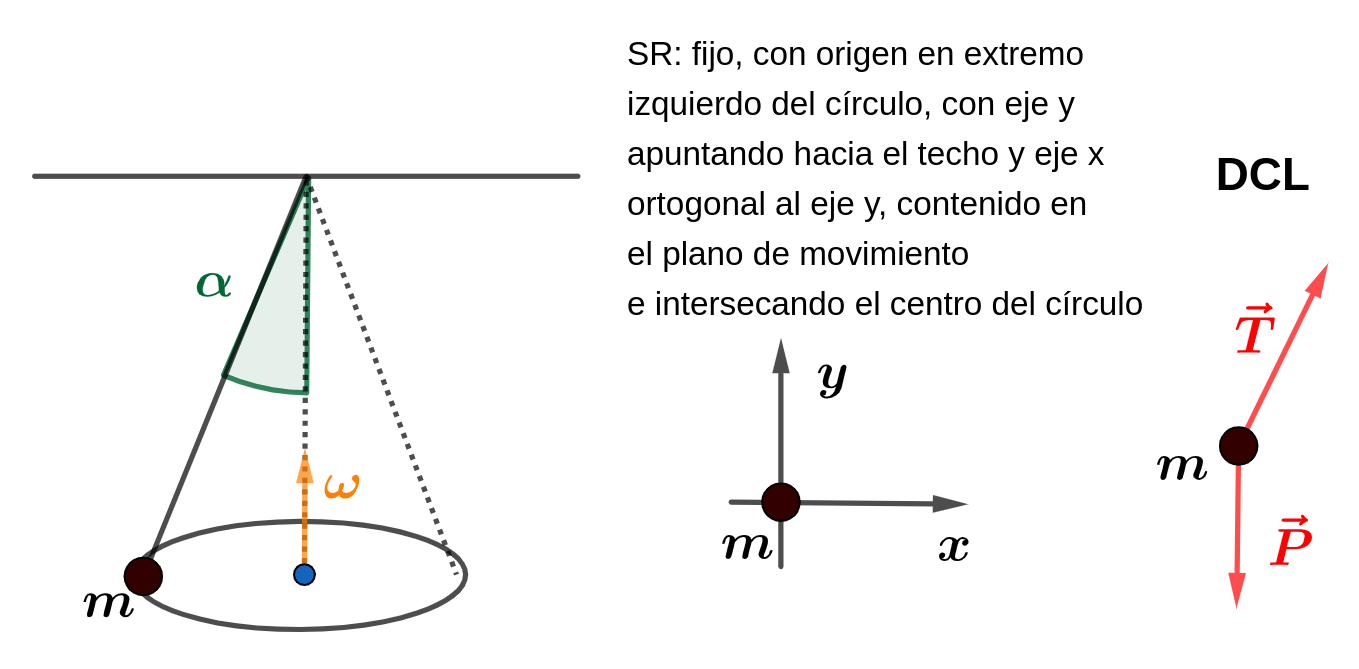
\includegraphics[scale=0.7]{../../common/img/62.01/theory/11-dynamics-conic-pendulum.png}
\label{fig:conic-pendulum}
\end{figure}

Por otro lado, dado que no hay pérdida de energía, el movimiento es infinito, por lo tanto $\alpha$ es constante y en consecuencia $\omega$ también. Con eso en mente, las ecuaciones de Newton resultan:

\begin{subequations}
\begin{align}
\textbf{x)} & \quad T \sin(\alpha) = m a_n \\
\textbf{y)} & \quad T \cos(\alpha) - P = 0
\end{align}
\end{subequations}

Ahora bien, si este mismo problema se plantea poniendo el sistema de referencia en el cuerpo suspendido del péndulo, el sistema pasa a ser no inercial. Cabe aclarar que en ese caso, el eje y seguiría apuntando al techo, en tanto el eje x pasaría a apuntar siempre hacia el centro del círculo. Por otro lado, el origen se movería siguiendo la posición del cuerpo. Teniendo en cuenta todo esto, el planteamiento pasa a ser el de la figura \ref{fig:conic-pendulum-ni}.

\begin{figure}[ht]
\centering
\caption{Péndulo cónico - SNI}
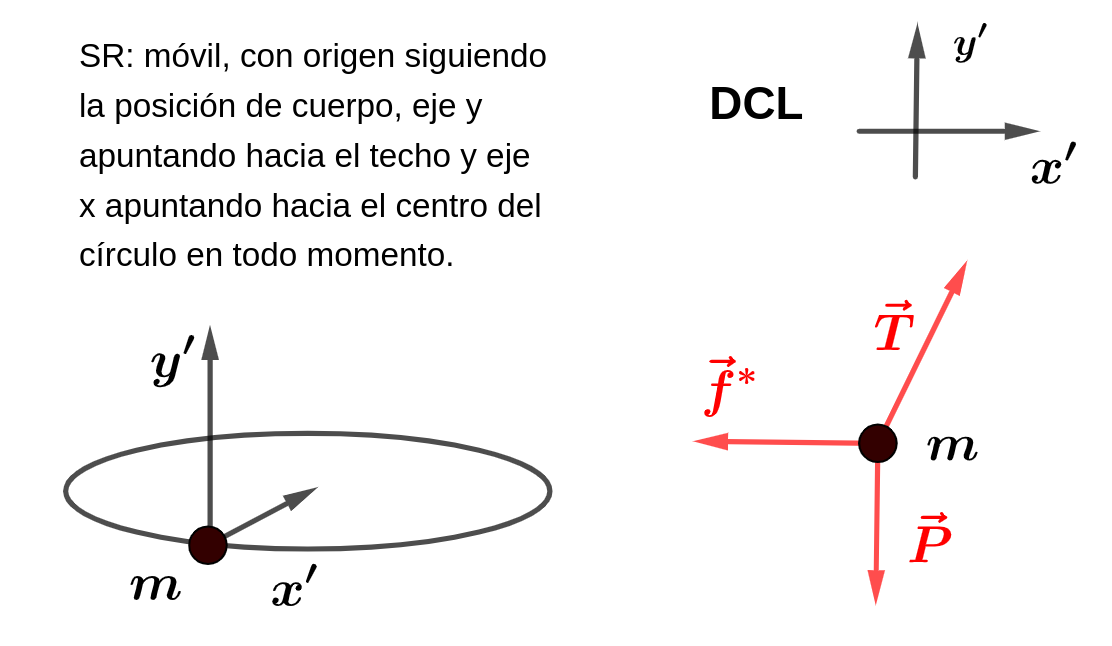
\includegraphics[scale=0.7]{../../common/img/62.01/theory/12-dynamics-conic-pendulum-ni.png}
\label{fig:conic-pendulum-ni}
\end{figure}

Nótese la aparición de la fuerza ficticia $\vec{f}^{*}$, en el sentido opuesto al de la aceleración centrífuga que experimenta el sistema de referencia. Dicha fuerza tendrá módulo igual a $m a_n$.

\subsubsection{Péndulo ideal}

Así como el péndulo cónico mueve el objeto suspendido en un plano horizontal, el péndulo ideal lo hace en un plano vertical, como se observa en la figura \ref{fig:ideal-pendulum}, en la cual, típicamente, se conocen el largo del hilo, $L$, y la masa del objeto, $m$. Para simplificar, el hilo se considera de masa despreciable comparada a la del objeto.

\begin{figure}[ht]
\centering
\caption{Péndulo ideal}
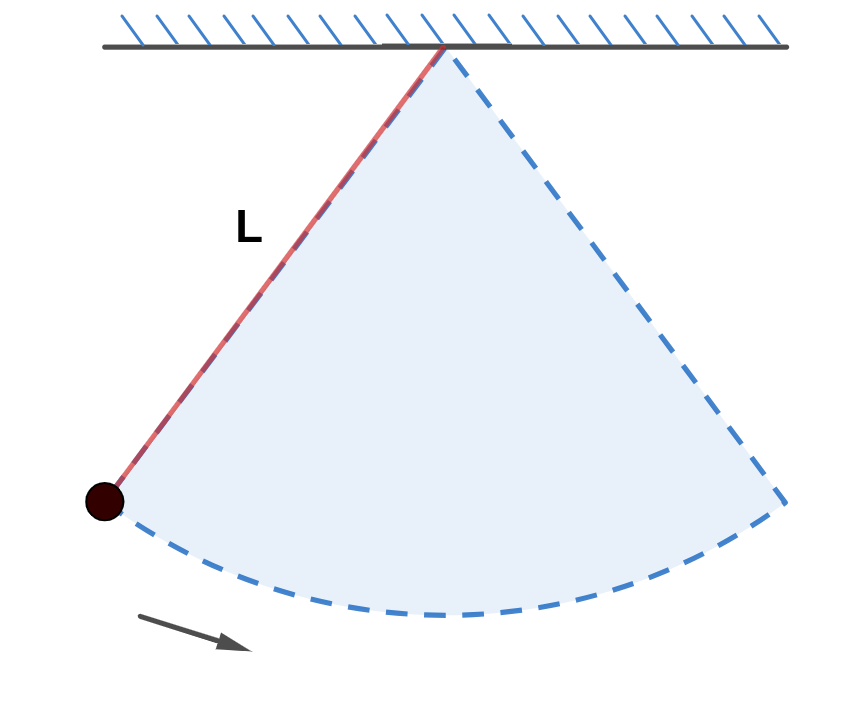
\includegraphics[scale=0.7]{../../common/img/62.01/theory/13-dynamics-ideal-pendulum.png}
\label{fig:ideal-pendulum}
\end{figure}

En un planteamiento no inercial, el sistema de referencia estaría en el objeto, con un sistema de coordenadas intrínseco: un eje en la direcciones normal y otro en la tangente, instante a instante. Esto conduciría a un diagrama de cuerpo libre como el de la figura \ref{fig:ideal-pendulum-ni}.

\begin{figure}[ht]
\centering
\caption{Péndulo ideal - SI}
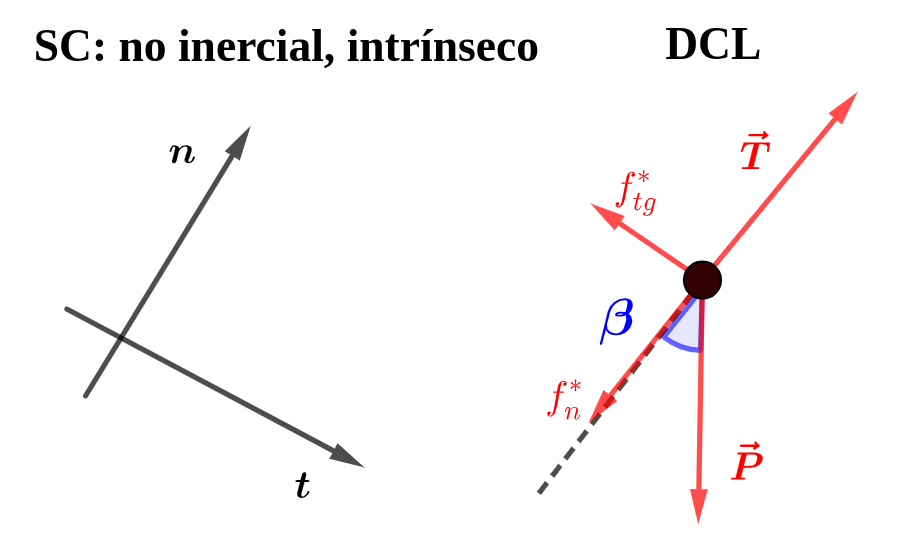
\includegraphics[scale=1]{../../common/img/62.01/theory/14-dynamics-ideal-pendulum-ni.png}
\label{fig:ideal-pendulum-ni}
\end{figure}

Con este sistema de referencia, el sistema de referencia presenta fuerzas ficticias en la dirección normal, y aceleración tangencial en la dirección homónima. Dichas fuerzas se oponen al sentido de la aceleración. Ello conduce a las siguientes ecuaciones de Newton:

\begin{subequations}
\begin{align}
\textbf{n)} & \quad T - P \cos(\beta) - m a_n = 0 \\
\textbf{t)} & \quad P \sin(\beta) - m a_{tg} = 0
\end{align}
\end{subequations}

Para resolver este sistema, lo más sencillo es tomar la ecuación tangencial y notar que el ángulo $\beta$ es congruente con el ángulo $\theta$ del péndulo, y por ende son iguales. Luego, $P = m g$. Y por último, $a_{tg}(t) = \frac{d^2s}{dt^2}$, donde $s$ es la posición del objeto medida a lo largo del arco de círculo (cero es la posición de equilibrio). Ello conduce a:

\begin{subequations}
\begin{align}
P \sin(\beta) - m a_{tg} = 0 \\
m g \sin(\theta) - m \frac{d^2s}{dt^2} = 0
\end{align}
\end{subequations}

Ahora bien, la posición en el arco está relacionado con $\theta$ y la longitud del hilo: $s = L \theta$. Derivando respecto al tiempo miembro a miembro dos veces, siendo $L$ una constante, resulta que $\frac{d^2s}{dt^2} = L \frac{d^2\theta}{dt^2}$. Reemplazando, se llega a una ecuación diferencial cuya incógnita es la función $\theta(t)$.

\begin{subequations}
\begin{align}
mg \sin(\theta) = m L \frac{d^2\theta}{dt^2} \\
\frac{d^2\theta}{dt^2} = \frac{g}{L} \sin(\theta)
\end{align}
\end{subequations}

Esta ecuación es bastante compleja para resolver de manera algebraica, dado que la función $\theta$ está compuesta con una función seno. Para simplificar, se puede plantear que para valores pequeños de $\theta$, $\sin(\theta) \approx \theta$. Ello conduce a una ecuación de 2do orden típica donde la solución general es una combinación lineal de un seno y coseno de cierta frecuencia.

\end{document}